%!TEX root = ../../Main.tex
\graphicspath{{Chapters/Opgave2/}}
%-------------------------------------------------------------------------------

\chapter{Lyd-afspilning/-optagelse}
For at kunne implementerer vores lyd afspilning og optagelse på crosscore var det først nødvendigt at eksportere vores, i opgave 1 beskrevede, frekvens sweep til en hex fil fra matlab. Denne fil, minFil.dat kunne vi derefter inkluderer i vores crosscore projekt og loade hex værdierne ind i et afspilningsarray. Dette er gjort med følgende kode.

\begin{figure}[H]
\centering
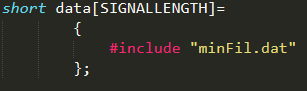
\includegraphics[width = 200pt]{Img/Inkluder.PNG}
\caption{Kode til at loade chirp ind i crosscore projekt}
\label{fig:Inkluder}
\end{figure}

Efter dette lavede vi en switchcase med udgangspunkt i det tidligere projekt med audioNotchFilteret. Det vil sige en switch med to cases. Første case PASSTHROUGH lod vi bare indgangen blive lig med udgangen på Blackfin'en. I den anden case ACTIVE, som aktiveres ved at trykke på en trykknap på Blackfin'en, lavede vi vores afspilning og optagelse af signalet. Ved hjælp af en counter, som inkrementeres ved hvert sample, holdte vi styr på at der kun afspiles så længe counteren var under længden af vores signal. Ligeledes holde counteren styr på at der kun optages så længe counteren var under længden af vores signal plus en buffer som vi definerede til at indeholde vores optagede signal.

\begin{figure}[H]
\centering
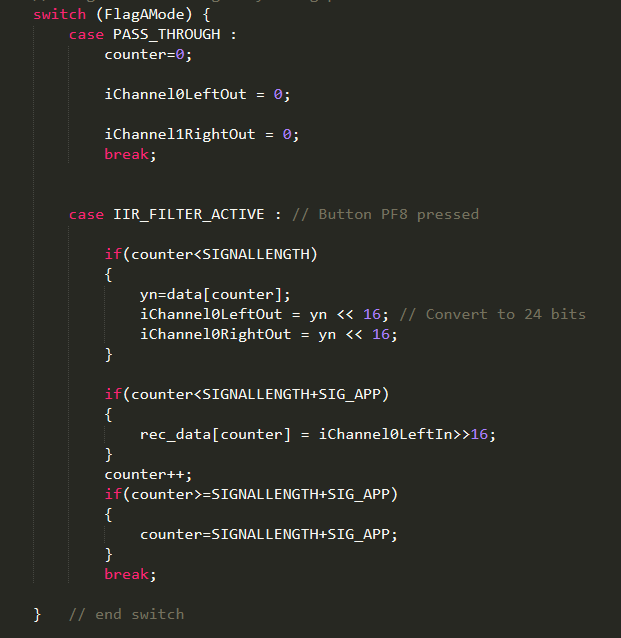
\includegraphics[width = 300pt]{Img/SwitchCase.PNG}
\caption{Kode til afspilning og optagelse på Blackfin}
\label{fig:SwitchCase}
\end{figure}

Efter optagelsen lå vores optagede data gemt i data\_rec arrayet. Dette array ønskede vi at eksportere således vi kunne behandle data'en i matlab. Til dette anvendete vi crosscore's indbyggede memorydump funktion som kunne eksportere dataen til en .dat fil som vi på samme måde som i opgave 1 kunne loade tilbage i matlab. Dataen blev eksporteret som floating point, signed fractional 16 bit, således det ikke var nødvendigt med en konvertering for at matlab kunne arbejde med dataen. Vi kunne altså direkte plotte vores modtagne signal i tidsdomænet i matlab efter indlæsning. 




